\documentclass{beamer}
\usepackage[spanish]{babel}
\usepackage[utf8]{inputenc}
\usepackage{graphicx}

\usecolortheme[RGB={122,59,122}]{structure}

\newtheorem{definicion}{Definición}
\newtheorem{ejemplo}{Ejemplo}

\title{Integración Trapecio \\ $f(x)=sen(\Pi x)$, $x \in [-2,-1]$}
\author{Lara Kristjansdottir, Javier Hernández Pérez}
\date{\today}
\usetheme{Madrid}
\begin{document}
\begin{frame}
  
\includegraphics[width=0.15\textwidth]{img/ullesc.eps}
  \hspace*{7.5cm}
  
\includegraphics[width=0.16\textwidth]{img/fmatesc.eps}
  \titlepage
  \begin{scriptsize}
    \begin{center}
    \title{Integración Trapecio de $f(x)=sen(\Pi x)$, $x \in [-2,-1]$}
      Facultad de Matemáticas \\Universidad de a Laguna
    \end{center}
  \end{scriptsize}
\end{frame}
%++++++++++++++++++++++++++++++++++++++++++++++++++++++++++++++++++++++++++++++++++++
%++++++++++++++++++++++++++++++++++++++++++++++++++++++++++++++++++++++++++++++++++++
\begin{frame}
  \frametitle{Contenido}
  \tableofcontents
\end{frame} 
%++++++++++++++++++++++++++++++++++++++++++++++++++++++++++++++++++++++++++++++++++++
%++++++++++++++++++++++++++++++++++++++++++++++++++++++++++++++++++++++++++++++++++++
\section{Motivación y objetivos}
\begin{frame}
\frametitle{Motivación}

El metodo de los trapecios y un terreno.
\end{frame}
% *************************************************************************************
\section{Descripción de los experimentos}
\begin{frame}
  \frametitle{Descripción}
  Vamos a aplicar la regla del trapecio a la función sin(pi*x) en el intervalo [-2,-1] utilizando una cantidad variable de subintervalos, n. Para cada valor de n, mediremos el error absoluto y el tiempo de ejecución del método.
\end{frame}

\section{Resultados obtenidos}
\begin{frame}
  \frametitle{Resultados}
  \begin{figure}[!th]
    \begin{center}
      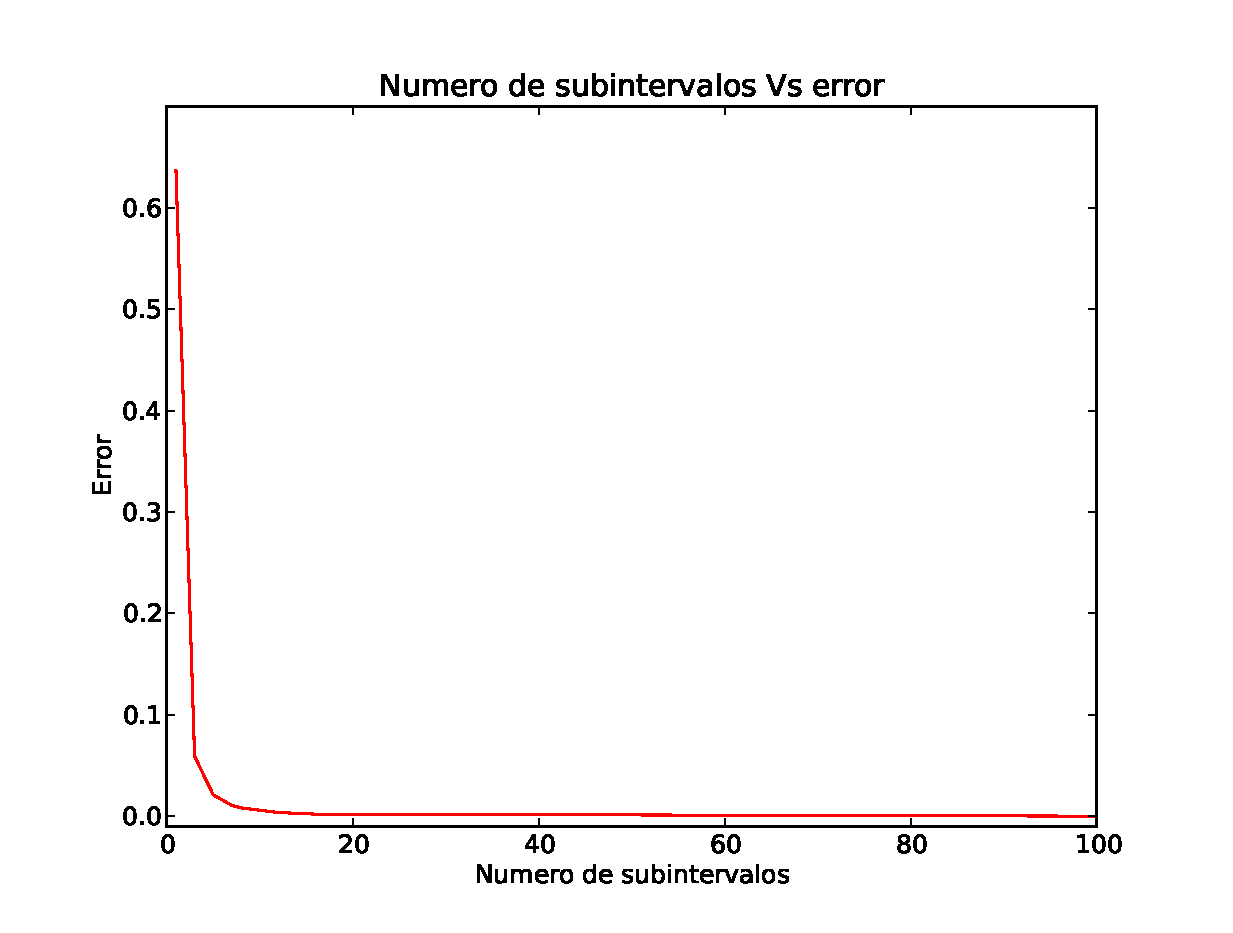
\includegraphics[width=0.75\textwidth]{img/Plot_nVSerror.eps}
      \caption{nVSerror}
      \label{fig:1}
    \end{center}
  \end{figure}
\end{frame}

\begin{frame}
  \frametitle{Resultados}
  \begin{figure}[!th]
    \begin{center}
      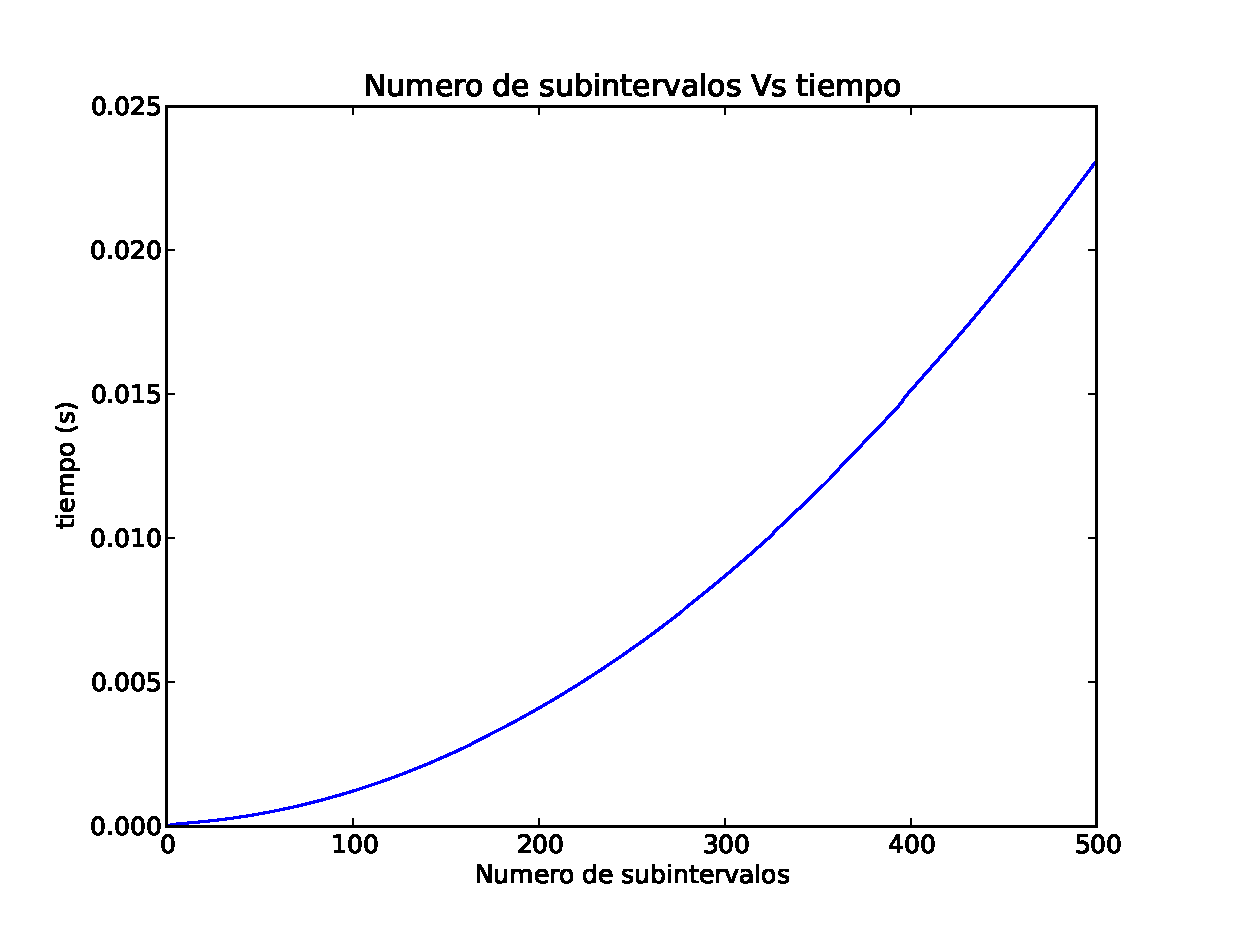
\includegraphics[width=0.75\textwidth]{img/Plot_nVStime.eps}
      \caption{nVStiempo}
      \label{fig:2}
    \end{center}
  \end{figure}
\end{frame}

%++++++++++++++++++++++++++++++++++++++++++++++++++++++++++++++++++++++++++++++  
\begin{frame}
  \frametitle{Bibliografía}

  \begin{thebibliography}{10}

    \beamertemplatebookbibitems
    \bibitem[libro]{libro}  
    Juan de Burgos Román (2007) Cálculo infinitesimal de una variable segunda edición McGraw Hill
    
    \beamertemplatebookbibitems
    \bibitem[\LaTeX]{latex}  
    http://www.latex-project.org/
    
    \beamertemplatebookbibitems
    \bibitem[Python]{python}  
    http://www.python.org/
    
      
    
      \end{thebibliography}
\end{frame}


%++++++++++++++++++++++++++++++++++++++++++++++++++++++++++++++++++++++++++++++  

\end{document}